% !TeX program = pdfLaTeX
\documentclass[12pt]{article}
\usepackage{amsmath}
\usepackage{graphicx,psfrag,epsf}
\usepackage{enumerate}
\usepackage{natbib}
\usepackage{textcomp}
\usepackage[hyphens]{url} % not crucial - just used below for the URL
\usepackage{hyperref}
\providecommand{\tightlist}{%
  \setlength{\itemsep}{0pt}\setlength{\parskip}{0pt}}

%\pdfminorversion=4
% NOTE: To produce blinded version, replace "0" with "1" below.
\newcommand{\blind}{0}

% DON'T change margins - should be 1 inch all around.
\addtolength{\oddsidemargin}{-.5in}%
\addtolength{\evensidemargin}{-.5in}%
\addtolength{\textwidth}{1in}%
\addtolength{\textheight}{1.3in}%
\addtolength{\topmargin}{-.8in}%

%% load any required packages here


\usepackage{color}
\usepackage{fancyvrb}
\newcommand{\VerbBar}{|}
\newcommand{\VERB}{\Verb[commandchars=\\\{\}]}
\DefineVerbatimEnvironment{Highlighting}{Verbatim}{commandchars=\\\{\}}
% Add ',fontsize=\small' for more characters per line
\usepackage{framed}
\definecolor{shadecolor}{RGB}{248,248,248}
\newenvironment{Shaded}{\begin{snugshade}}{\end{snugshade}}
\newcommand{\KeywordTok}[1]{\textcolor[rgb]{0.13,0.29,0.53}{\textbf{#1}}}
\newcommand{\DataTypeTok}[1]{\textcolor[rgb]{0.13,0.29,0.53}{#1}}
\newcommand{\DecValTok}[1]{\textcolor[rgb]{0.00,0.00,0.81}{#1}}
\newcommand{\BaseNTok}[1]{\textcolor[rgb]{0.00,0.00,0.81}{#1}}
\newcommand{\FloatTok}[1]{\textcolor[rgb]{0.00,0.00,0.81}{#1}}
\newcommand{\ConstantTok}[1]{\textcolor[rgb]{0.00,0.00,0.00}{#1}}
\newcommand{\CharTok}[1]{\textcolor[rgb]{0.31,0.60,0.02}{#1}}
\newcommand{\SpecialCharTok}[1]{\textcolor[rgb]{0.00,0.00,0.00}{#1}}
\newcommand{\StringTok}[1]{\textcolor[rgb]{0.31,0.60,0.02}{#1}}
\newcommand{\VerbatimStringTok}[1]{\textcolor[rgb]{0.31,0.60,0.02}{#1}}
\newcommand{\SpecialStringTok}[1]{\textcolor[rgb]{0.31,0.60,0.02}{#1}}
\newcommand{\ImportTok}[1]{#1}
\newcommand{\CommentTok}[1]{\textcolor[rgb]{0.56,0.35,0.01}{\textit{#1}}}
\newcommand{\DocumentationTok}[1]{\textcolor[rgb]{0.56,0.35,0.01}{\textbf{\textit{#1}}}}
\newcommand{\AnnotationTok}[1]{\textcolor[rgb]{0.56,0.35,0.01}{\textbf{\textit{#1}}}}
\newcommand{\CommentVarTok}[1]{\textcolor[rgb]{0.56,0.35,0.01}{\textbf{\textit{#1}}}}
\newcommand{\OtherTok}[1]{\textcolor[rgb]{0.56,0.35,0.01}{#1}}
\newcommand{\FunctionTok}[1]{\textcolor[rgb]{0.00,0.00,0.00}{#1}}
\newcommand{\VariableTok}[1]{\textcolor[rgb]{0.00,0.00,0.00}{#1}}
\newcommand{\ControlFlowTok}[1]{\textcolor[rgb]{0.13,0.29,0.53}{\textbf{#1}}}
\newcommand{\OperatorTok}[1]{\textcolor[rgb]{0.81,0.36,0.00}{\textbf{#1}}}
\newcommand{\BuiltInTok}[1]{#1}
\newcommand{\ExtensionTok}[1]{#1}
\newcommand{\PreprocessorTok}[1]{\textcolor[rgb]{0.56,0.35,0.01}{\textit{#1}}}
\newcommand{\AttributeTok}[1]{\textcolor[rgb]{0.77,0.63,0.00}{#1}}
\newcommand{\RegionMarkerTok}[1]{#1}
\newcommand{\InformationTok}[1]{\textcolor[rgb]{0.56,0.35,0.01}{\textbf{\textit{#1}}}}
\newcommand{\WarningTok}[1]{\textcolor[rgb]{0.56,0.35,0.01}{\textbf{\textit{#1}}}}
\newcommand{\AlertTok}[1]{\textcolor[rgb]{0.94,0.16,0.16}{#1}}
\newcommand{\ErrorTok}[1]{\textcolor[rgb]{0.64,0.00,0.00}{\textbf{#1}}}
\newcommand{\NormalTok}[1]{#1}

\usepackage{longtable}
\usepackage{booktabs}

\begin{document}


\def\spacingset#1{\renewcommand{\baselinestretch}%
{#1}\small\normalsize} \spacingset{1}


%%%%%%%%%%%%%%%%%%%%%%%%%%%%%%%%%%%%%%%%%%%%%%%%%%%%%%%%%%%%%%%%%%%%%%%%%%%%%%

\if0\blind
{
  \title{\bf Can a deep learning model read residual plots?}

  \author{
        Shuofan Zhang \thanks{The authors gratefully acknowledge \ldots{}} \\
    Master student, Monash University\\
     and \\     Di Cook \\
    Professor of Business Analytics\\
      }
  \maketitle
} \fi

\if1\blind
{
  \bigskip
  \bigskip
  \bigskip
  \begin{center}
    {\LARGE\bf Can a deep learning model read residual plots?}
  \end{center}
  \medskip
} \fi

\bigskip
\begin{abstract}
Residuals plots are a primary means to diagnose statistical models. It
requires human evaluation to determine if the structure in the plot is
consistent with a random variation or not. If not, then the diagnosis is
that the model has not adequately captured the relationships between
response and explanatory variable in the data. This thesis develops a
computer vision model to read residual plots. It compares results with a
large database of human evaluations. The evaluations were conducted
using a protocol called the ``lineup'' which places residual plots in a
formal framework for statistical hypothesis testing. The comparison
between computer and human is made on a very restricted and controlled
set of residual plot structures. A new small human subject study is also
conducted to compare human vs.~computer in reading heteroscedasticity.
\end{abstract}

\noindent%
{\it Keywords:} model diagnosis, computer vision
\vfill

\newpage
\spacingset{1.45} % DON'T change the spacing!

\section{Introduction}
\label{sec:intro}

``The multiple regression model for cross-sectional data is still the
most widely used vehicle for empirical analysis in economics and other
social sciences'' \citep{IE17}. Detecting possible violations of the
Gauss-Markov assumptions is crucial to interpreting the data properly,
especially in the early stage of analysis. There are several
distribution tests that are commonly used, for instance, the Pearson
correlation test for detecting linear relationship; the Breusch-Pagan
test and White test for investigating heteroskedasticity. But primarily
residual plots are the main diagnostic tool and these rely on human
evaluation. Because data plots show a lot more information than a single
statistic. A good example here would be Anscombe's Quartet. ``It is a
set of four distinct data sets each consisting of 11 (x,y) pairs where
each dataset produces the same summary statistics (mean, standard
deviation, and correlation) while producing vastly different plots''
\citep{ANS73}. Matejka and Fitzmaurice also did an interesting study on
this issue, they used `datasaurus' data from \citet{DS16} and generated
a series of data with same statistics but very different plots as shown
in figure \ref{fig:saurus}. \citep{JM17}

\begin{figure}
\centering
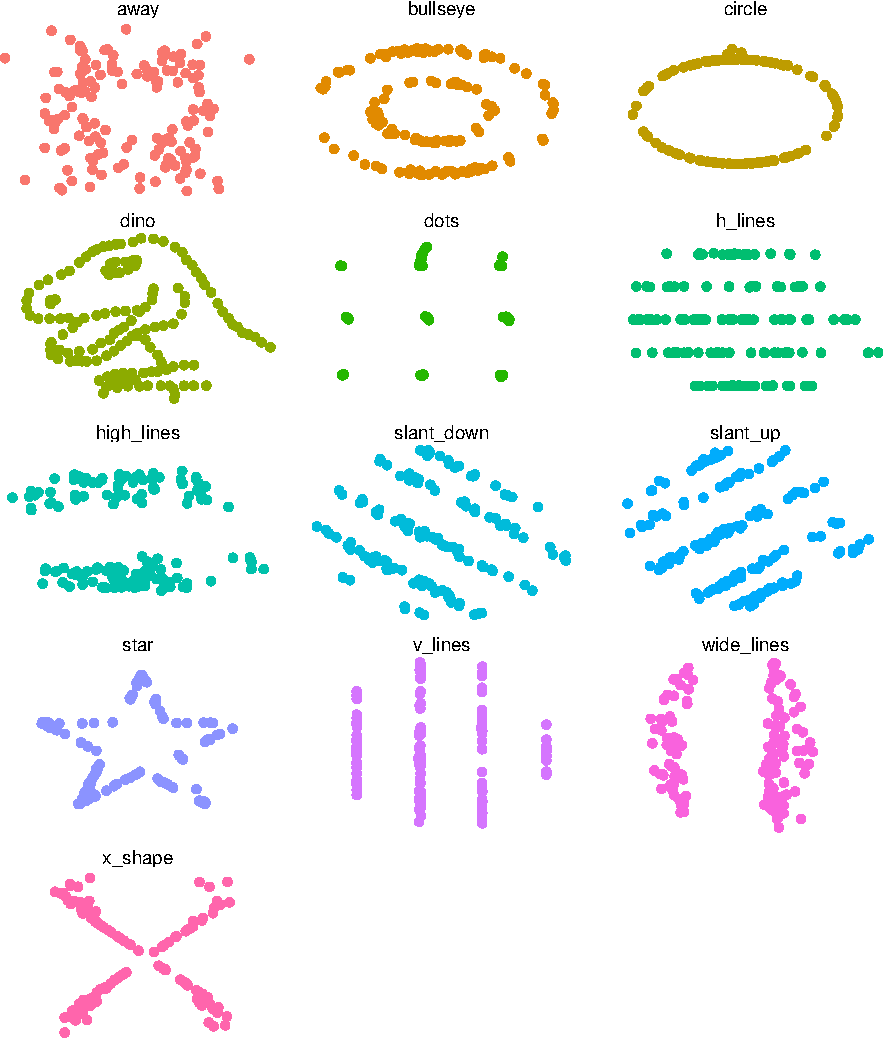
\includegraphics{pc_plots_files/figure-latex/saurus-1.pdf}
\caption{Each dataset has the same summary statistics to two decimal
places: (E(x)=54.26, E(y)=47.83, Pearson's r=, sd(x)=16.76, sd(y)=26.93}
\end{figure}

Steps of constructing computer experiment are discussed in section 2,
Turk study (human evaluation) is explained. Section 3 compares computer
performance against the database of human evaluation in reading linear
relationship. Section 4 contains a short summary and some discussion
regarding the future study.

Former studies have shown that human eyes are sensitive to the
systematic patterns in data plots. With proper manipulation, visualized
plots can be used as test statistics and perform a valid hypothesis
test. One example of these protocols that provides inferential validity
is called ``lineup'' which is introduced by \citet{HW10}. ``The protocol
consists of generating 19 null plots (could be other numbers), inserting
the plot of the real data in a random location among the null plots and
asking the human viewer to single out one of the 20 plots as most
different from the others'' \citep{HW10}. If the real plot is chosen, it
means the real data is likely to be different from the null hypothesis,
so we reject the null hypothesis with 5\% chance to be wrong (Type I
error). Because if all 20 plots are generated from the null
distribution, the chance of one plot being picked is \(1/20\) which is
5\%. With the assistance of ``lineup'', we avoid falling into the trap
of apophenia where we see patterns in random noise. This protocol has
proved to be valid and powerful theoretically as well as practically
through human experiments, especially when the assumptions for doing
conventional tests are violated \citep{MM13}. The human factors that may
influence visual statistical inference were also investigated by
\citet{human2014}. The experiments in \citet{human2014} suggest that
``individual skills vary substantially, but demographics do not have a
huge effect on performance.'' Although there are some statistically
significant factors such as ``having a graduate degree'' and ``living
country'', the effects of these factors are minimal. These results
demonstrate the robustness of the test against different human factors.
Figure \ref{fig:lineup} is an example of the lineup. Which plot do you
think is the most different? If you choose plot one, we are 95\%
confident to reject the no-relationship assumption between the two
variables, ``hp'' and ``disp'' \citep{SIM18}. The lineup protocol can
also be used for other types of testing by choosing different types of
plot. For example, normality can be tested using QQ plot; the difference
in mean can be tested using box plot; etc.

The question that arises today is whether we can train a computer to
read residual plot and make relevant decisions, particularly with a
computer vision approach such as deep learning. If this is feasible, we
can have the deep learning model process a lot more data than a human
can manage. Thus, the cost of rendering visual inference will become
much lower.

\begin{figure}
\centering
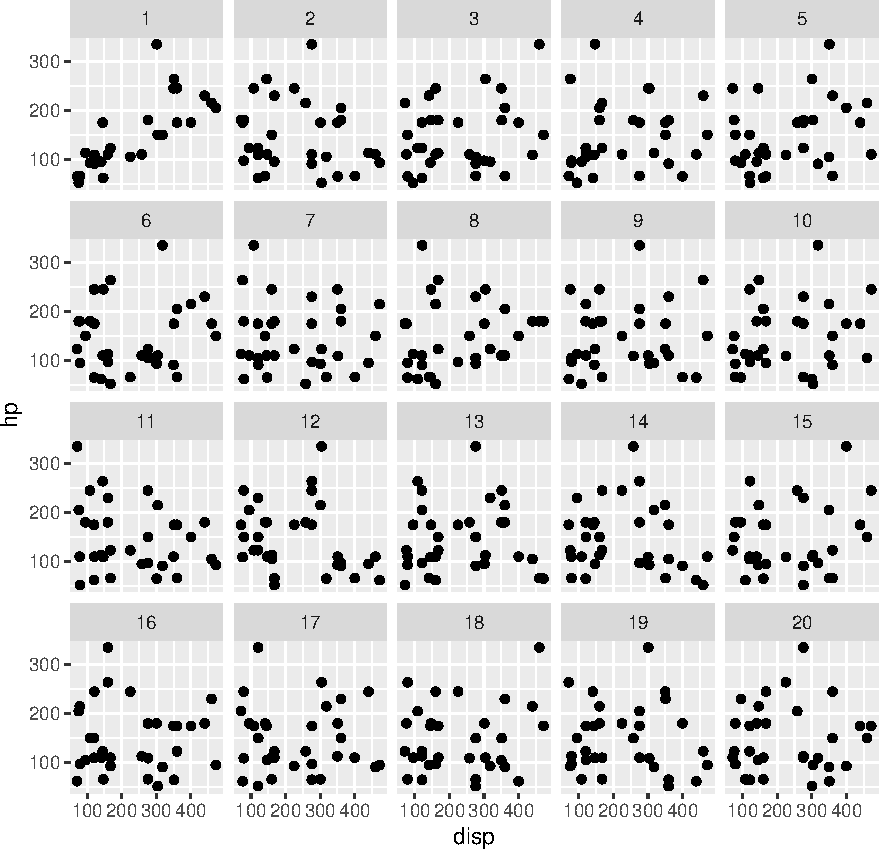
\includegraphics{pc_plots_files/figure-latex/lineup-1.pdf}
\caption{Scatterplot lineup example: one plot is the data, the rest are
generated from a null model assuming no relationship between the two
variables. In this lineup it is easy to see that plot 1, which is the
data plot, is different from the rest.}
\end{figure}

The motivation for the task is provided in a blog post by Giora Simchoni
\citep{SIM18}. He has designed a deep learning model to test the
significance of the linear relationship between two variables for
samples of size 50. The model reached over 93\% accuracy on unseen test
data. He also mentioned that the computer fails to pick up a strong
non-linear relationship even though the Pearson'r is as high as -0.84
\citep{SIM18}. So the short conclusion is the computer vision is not
perfect, in that it is not as flexible as human vision. As Simchoni
explained in his article, the model can only distinguish linear
relationship from no-relationship as trained. However, we think this
fact is just another example reflecting the importance of visualization
as we discussed above. A strong correlation does not necessarily mean a
linear relationship. We should always refer to the plot before making
any statement. What's more, if we want the model to be more flexible, we
could simply adjust our design of training accordingly. Therefore, in
this article, we are trying to further Simchoni's study. More
specifically, we will build a computer model to perform the hypothesis
tests as follows. The hypothesis test is:

\(H_0\): There are no relationships between the two variables.

\(H_1\): There is a linear relationship between the two variables where
all Gauss-Markov assumptions are met. For ease of exposition, only the
regression model with one explanatory variable will be considered in
this paper, but many of the results can be generalized to other cases
including multiple regression model. Because the ``statistics'' we will
use is the scatterplot, in terms of teaching the computer reading the
plot, one variable is enough to generate different patterns in that plot
for the deep learning model to learn. And this makes the design process
much simpler.

The model we will use is the convolutional neural networks, also known
as convnets, a type of deep-learning model ``almost universally used in
computer vision applications'' \citep{DLR18}. The very first
convolutional neural networks, called the ``LeNet5'' which was born in
1994, propelled the field of deep learning. However, this technique was
in incubation from 1998 to 2010. In recent years, with the increasing
data availability and more advanced technology, the design of the neural
network architecture became more and more successful. Many types of
neural network architectures have been developed since then, such as the
``Dan Ciresan Net'' which enabled the implementation of GPU for the
first time, and the ``AlexNet'' which used the so-called ``ReLU''
function as the activation function and started a small revolution in
the deep learning world, etc. \citep{cnn2017} Basically convolutional
neural networks has two interesting properties: ``the patterns they
learn are translation invariant'', and ``they can learn spatial
hierarchies of patterns'' \citep{DLR18}. The first property implies that
once the model learns how to recognize the linear patterns, it can
detect these patterns regardless of their direction, thus handling
negative/positive relationship automatically in our case.

Unlike the classical programming where human input rules, in deep
learning paradigm, we provide data and the answers associated with the
data. Deep learning algorithm will output the rules, and these rules can
then be used on new data to make predictions. To make our life easier,
we can also think of the deep learning neural network as a complex
nonlinear model which could estimate millions of parameters
(\(\textbf{w}\)) with a big enough dataset. As usual regression problem,
to get the estimates of unknown parameters (\(\textbf{w}\)), we need to
provide the model with the dependent variable (\(y_i\)) and the
independent variables (\(\textbf{x}_i\)). In this case, the independent
variable will be the images of data plots (in forms of matrices)
simulated from the null distribution and the alternative distribution,
and dependent variable will be the labels of that plot indicating the
true relationship of the original data. Once we have the estimated
parameters (\(\hat{\textbf{w}}\)), we then can use them to classify
unseen data plots, e.g.~to perform a hypothesis test.

The architecture used in this study is a fundamental one. The estimation
method for the deep-learning model is called ``backpropagation''
algorithm which is a way to train chains of parametric operations using
gradient-descent optimization. The gradient-descent optimizer is meant
to find the set of parameters such that the cost function reaches its
minimum. The form of the cost functions or loss function is determined
per each question. In both two experiments conducted in this paper, the
deep learning model is expected to complete binary classification task,
e.g.~tell ``linearly correlated'' variables from ``independent''
variables for the first experiment, tell ``heteroskedasticity errors''
from ``normal errors'' for the second experiment. As introduced by
\citet{DLR18}, ``crossentropy is usually the best choice (as the loss
function) when you're dealing with models that output probabilities''.
Originated from Information Theory, crossentropy is a quantity measuring
the distance between probability distributions. In deep learning world,
it measures the distance between the true distribution and the
predictions. Therefore, in this paper, the binary crossentropy loss
function will be used. The associated cost function is of the form,
\[J(\textbf{w})=- \frac{1}{N}\sum_{i=1}^N\left(  
\ y_i\ log\hat{y_i}+(1-y_i)\ log(1-\hat{y_i})  
\right)\] where
\(\hat{y_i} = g(\textbf{w} \times \textbf{x}_i) = \frac{1}{1+e^{-\textbf{w} \times \textbf{x}_i}}\)
and \(g(z)\) is the logistic function.

The main procedures involved in constructing and selecting a convnets
model are shown in figure \ref{dgpc}. The convnets is trained on
``train'' and ``validation'' set. A certain number of iterations over
all samples are done, the fitted convnets given by each iteration are
saved, one best model is chosen as the representative for the computer
according to the overall accuracy on the unseen ``test'' set.

The main procedures of the human evaluating lineup are given in figure
\ref{dghm}. ``Real data'' and ``null data'' stand for datasets simulated
under the alternative hypothesis and the null hypothesis respectively.

\begin{figure*}[h]
\centerline{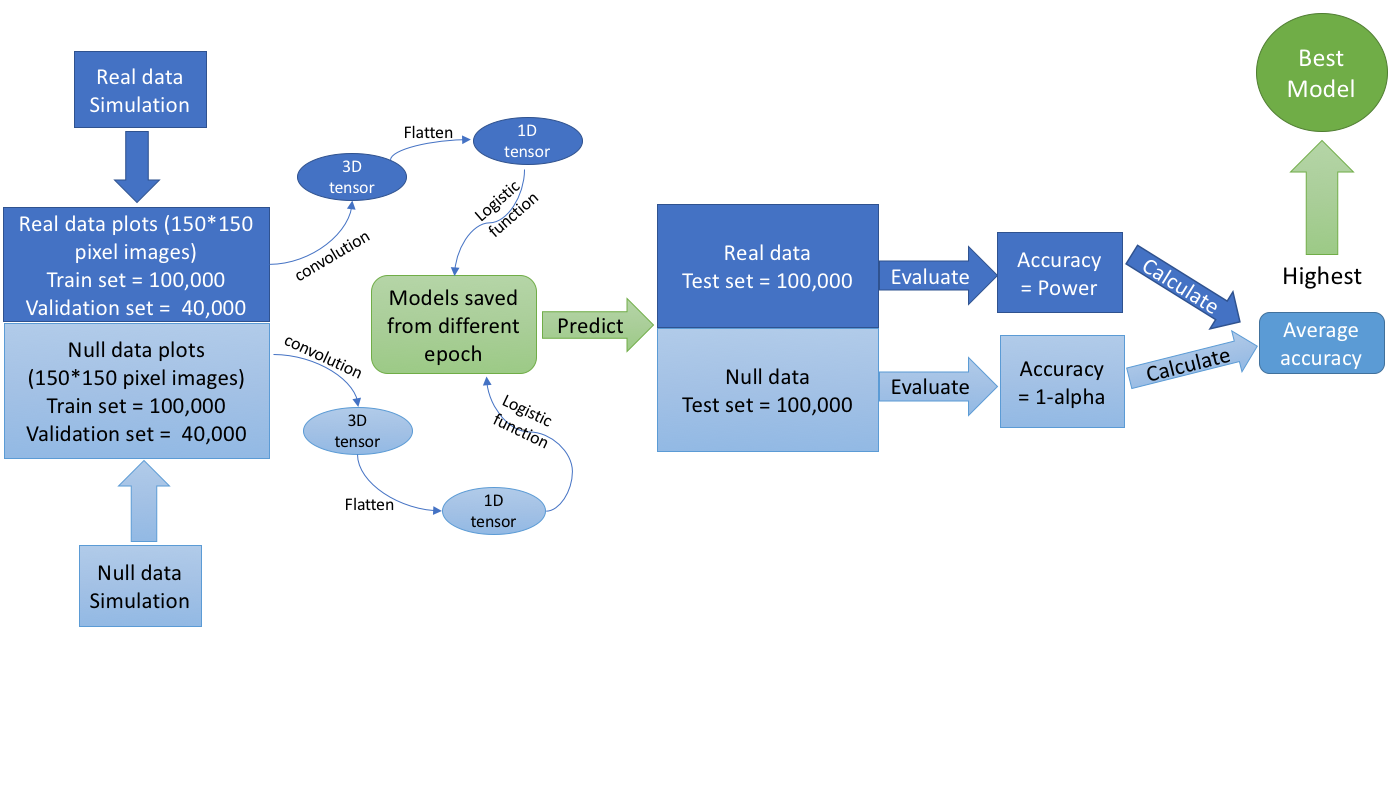
\includegraphics[width=15cm]{figures/diagpc.png}}
\caption{Diagram illustrating the training, diagnosis and choice of the computer model. Based on 480,000 simulated data sets used to create $150\times 150$ pixel images, divided into train, validation and test sets.}
\label{dgpc}
\end{figure*}

\begin{figure*}[h]
\centerline{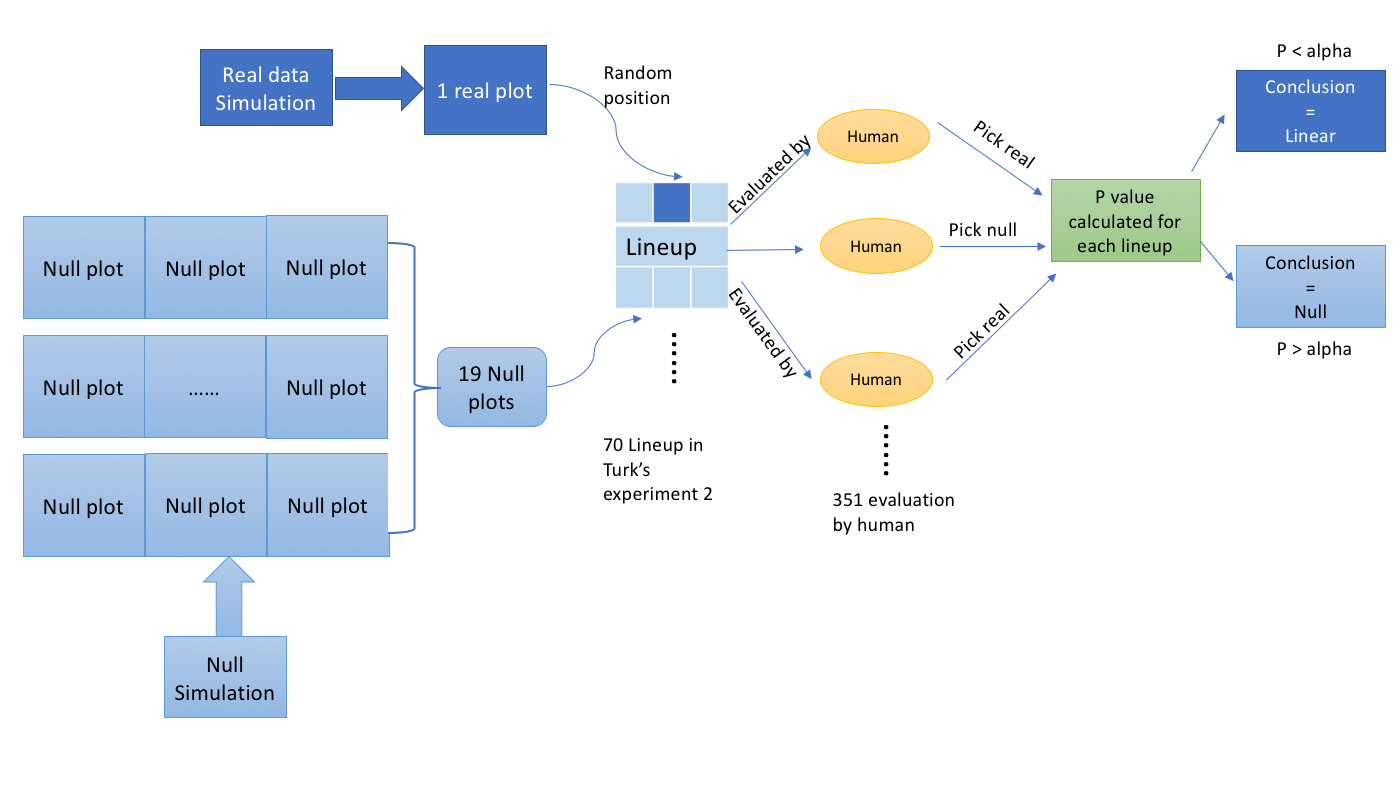
\includegraphics[width=15cm]{figures/diaghm.png}}
\caption{Diagram illustrating the process of human subject evaluation of lineups, and how performance is computed.}
\label{dghm}
\end{figure*}

\section{Experimental Methods}
\label{sec:experiment}

\subsection{Comparing computer performance against the database of human
evaluation}\label{comparing-computer-performance-against-the-database-of-human-evaluation}

A database of human evaluations of scatterplots is available from prior
studies. This is used to compare the performance of the computer model.
The computer model is trained on a broader parameter simulation
framework and tested on the same data as the human evaluations.

\subsubsection{Amazon Mechanical Turk
study}\label{amazon-mechanical-turk-study}

\begin{figure*}[h]
\centerline{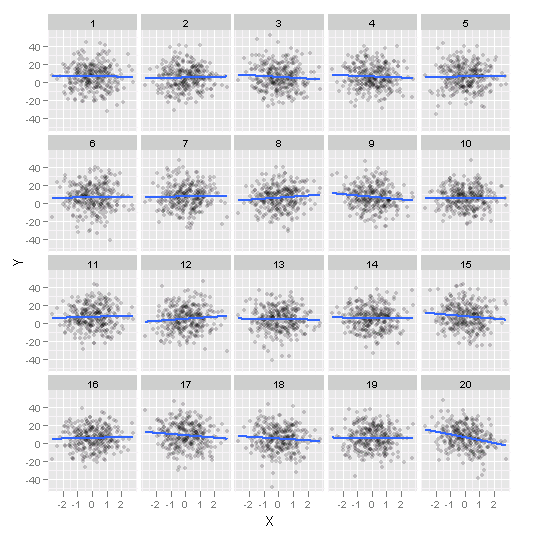
\includegraphics[width=15cm]{figures/plot_turk2_300_350_12_3.png}}
\caption{One of 70 lineups used in experiment 2 Majumder et al (2012). Of the 65 people who examined the lineup,  63 selected the data plot, which is in position 20.}
\label{expt2}
\end{figure*}

A large database of results from human subjects was collected examine
the performance of the lineup protocol relative to classical tests. The
work is published in \citet{MM13}. This database forms the basis of the
test set used to examine the computer model performance.

In \citet{MM13}, ``three experiments were conducted to evaluate the
effectiveness of the lineup protocol relative to the equivalent test
statistic used in the regression setting.'' In each experiment, they
simulated data from a controlled setting and then generated associated
lineup for the human to evaluate. The human subjects were hired from
Amazon Mechanical Turk where is a marketplace for work that requires
human intelligence. \citep{amazon}

The controlled model in their first experiment is
\[Y_i=\beta_0+\beta_1 X_{i1}+\beta_2 X_{i2}+\epsilon_i\] where
\(\beta_0=5, \beta_1=15, X_1 \sim Poisson(\lambda=30), \epsilon_i\sim N(0,\sigma^2), i=1,2,...,n\),
\(\beta_2\) used in generating real data is specified in table 2.1.
While in the null model \(\beta_2=0\), and the null data was generated
by simulating from \(N(0,\hat{\sigma}^2)\). This experiment was aimed to
test the ability of human on detecting the effect of \(X_2\).

Their second experiment is very similar to the first one, but there is
only one continuous variable \(X_1\) on the right-hand side. It examined
the performance of humans in recognising linear association between two
variables, in direct comparison to conducting a \(t\)-test of
\(H_o: \beta_k=0\) vs \(H_a: \beta_k\neq 0\) assessing the importance of
including variable \(k\) in the linear model. The actual data model is
\[Y_i=\beta_0+\beta_1 X_{i1}+\epsilon_i\] where
\(\beta_0=6, X_1\sim N(0,1)\), and the null data was generated from
\(N(0, \hat{\sigma}^2)\).

The third experiment in their paper contains contaminated data where the
actual data were in fact generated from two different specifications.
\[Y_i=
  \begin{cases}
    \alpha+\beta X_i+\epsilon_i       & \quad X_i\sim N(0,1)\ \ i=1,...,n\\
    \lambda+\eta_i  & \quad X_i\sim N(\mu,1/3)\ \ i=1,...,n_c
  \end{cases}
\] where
\(\epsilon_i \sim N(0,\sigma), \eta_i \sim N(0,\sigma/3), \ \mu=-1.75, \ \beta\in(0.1, 0.4, 0.75, 1.25, 1.5, 2.25)\).
And \(n=100, n_c=15, alpha=0, \lambda=10, \sigma=3.5\). The null plots
were generated from \(N(0,\hat{\sigma}^2)\).

Other parameters in the ``actual'' data sets of Turk experiment one and
Turk experiment two are shown in table 2.1. In this study, we will
mainly focus on their second experiment and use its database to form our
first comparison experiment. This experiment 2 utilized 70 lineups of
size 20 plot, with varying degrees of departure from the
\(H_o: \beta_k=0\). There were 351 evaluations by human subjects. These
results will be used for comparison with the deep learning model. An
example lineup question in Turk experiment 2 is shown in Figure
\ref{expt2}. For this lineup, 63 of the 65 people who examined it
selected the data plot (position 20) from the null plots. There is clear
evidence that the data displayed in plot 20 is not from
\(H_o: \beta_k=0\).

\begin{longtable}[]{@{}ccc@{}}
\caption{Combination of parameter values used for simulation in Turk's
study. (continued below)}\tabularnewline
\toprule
\begin{minipage}[b]{0.23\columnwidth}\centering\strut
Sample size (n)\strut
\end{minipage} & \begin{minipage}[b]{0.23\columnwidth}\centering\strut
Error SD(sigma)\strut
\end{minipage} & \begin{minipage}[b]{0.25\columnwidth}\centering\strut
Experiment 1 beta2\strut
\end{minipage}\tabularnewline
\midrule
\endfirsthead
\toprule
\begin{minipage}[b]{0.23\columnwidth}\centering\strut
Sample size (n)\strut
\end{minipage} & \begin{minipage}[b]{0.23\columnwidth}\centering\strut
Error SD(sigma)\strut
\end{minipage} & \begin{minipage}[b]{0.25\columnwidth}\centering\strut
Experiment 1 beta2\strut
\end{minipage}\tabularnewline
\midrule
\endhead
\begin{minipage}[t]{0.23\columnwidth}\centering\strut
100\strut
\end{minipage} & \begin{minipage}[t]{0.23\columnwidth}\centering\strut
5\strut
\end{minipage} & \begin{minipage}[t]{0.25\columnwidth}\centering\strut
0,1,3,5,8\strut
\end{minipage}\tabularnewline
\begin{minipage}[t]{0.23\columnwidth}\centering\strut
100\strut
\end{minipage} & \begin{minipage}[t]{0.23\columnwidth}\centering\strut
12\strut
\end{minipage} & \begin{minipage}[t]{0.25\columnwidth}\centering\strut
1,3,8,10,16\strut
\end{minipage}\tabularnewline
\begin{minipage}[t]{0.23\columnwidth}\centering\strut
300\strut
\end{minipage} & \begin{minipage}[t]{0.23\columnwidth}\centering\strut
5\strut
\end{minipage} & \begin{minipage}[t]{0.25\columnwidth}\centering\strut
0,1,2,3,5\strut
\end{minipage}\tabularnewline
\begin{minipage}[t]{0.23\columnwidth}\centering\strut
300\strut
\end{minipage} & \begin{minipage}[t]{0.23\columnwidth}\centering\strut
12\strut
\end{minipage} & \begin{minipage}[t]{0.25\columnwidth}\centering\strut
1,3,5,7,10\strut
\end{minipage}\tabularnewline
\bottomrule
\end{longtable}

\begin{longtable}[]{@{}c@{}}
\toprule
\begin{minipage}[b]{0.40\columnwidth}\centering\strut
Experiment 2 beta1\strut
\end{minipage}\tabularnewline
\midrule
\endhead
\begin{minipage}[t]{0.40\columnwidth}\centering\strut
0.25, 0.75, 1.25, 1.75, 2.75\strut
\end{minipage}\tabularnewline
\begin{minipage}[t]{0.40\columnwidth}\centering\strut
0.5, 1.5, 3.5, 4.5, 6\strut
\end{minipage}\tabularnewline
\begin{minipage}[t]{0.40\columnwidth}\centering\strut
0.1, 0.4, 0.7, 1, 1.5\strut
\end{minipage}\tabularnewline
\begin{minipage}[t]{0.40\columnwidth}\centering\strut
0, 0.8, 1.75, 2.3, 3.5\strut
\end{minipage}\tabularnewline
\bottomrule
\end{longtable}

\subsubsection{Linear relationship
simulation}\label{linear-relationship-simulation}

The design for our model under the alternative hypothesis in the first
experiment is similar to what \citet{SIM18} did in his blog. But the
parameters are tailored to compare the computer performance with the
Turk study results.

The model under the alternative is designed as:
\[Y_i = \beta_0 + \beta_1 X_{i}  + \varepsilon_i, ~~i=1, \dots , n\] And
all the parameters in our model were designed to cover the range used in
the second experiment in Turk study \citep{MM13}. Therefore, the
relevant parameters in our model are generated using the following
specification.

\begin{itemize}
\item
  \(X \sim N[0,\ 1]\)\\
  Distributions of X has an impact on the shape of the scatters. For
  instance, if X is generated from a uniform distribution, then the
  plots will look like a square when the sample size is large; while
  looking like a circle if X follows a normal distribution.
\item
  \(\beta_0 = 0\)\\
  Intercept is arbitrarily set to be zero because it has no impact on
  the patterns in the data plots.
\item
  \(\beta_1\sim U[-10, -0.1] \bigcup [0.1, 10]\)\\
  \(\beta_1\) is designed to be uniformly generated from -10 to 10
  (excluding -0.1 to 0.1).
\item
  \(\varepsilon\sim N(0, \sigma^2) \ where\ \sigma \sim U[1,12]\)\\
  \(\varepsilon\) is designed to be uniformly distributed from 1 to 12.
\item
  \(n=U[50,500]\)\\
  The sample sizes of each data set vary from 50 to 500 observations.
\end{itemize}

Figure \ref{fig:linear} shows four example plots generated using the
specifications above. To facilitate the computer vision, all texts,
ticks, and titles of X and Y axes are removed, so does the background
grid. Under this controlled structure, a total number of 240,000
datasets are simulated. Figure \ref{fig:simplot} contains a histogram of
the simulated n, a histogram of the simulated \(\beta\), a histogram of
the simulated \(\sigma\), a histogram of the estimated sample p-value, a
scatter plot of \(\beta\) against n and a scatter plot of \(\sigma\)
against n. These plots show good coverage over the alternative parameter
space.

\begin{figure}
\centering
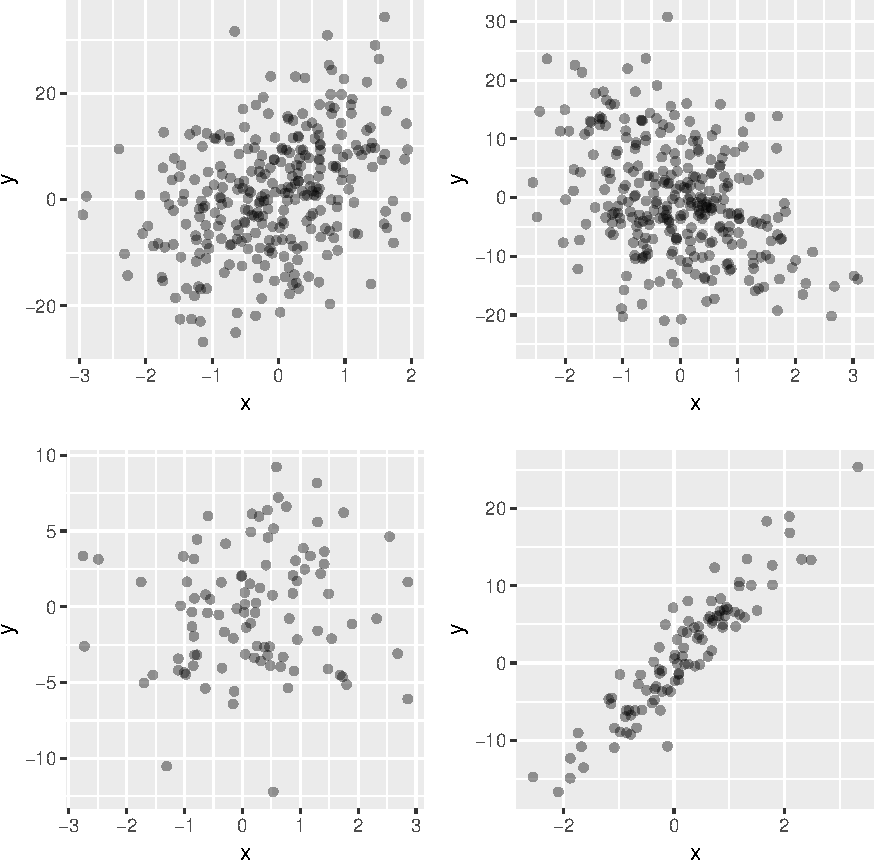
\includegraphics{pc_plots_files/figure-latex/linear-1.pdf}
\caption{Four examples of data plots generated from the classic linear
model.}
\end{figure}

\begin{figure}
\centering
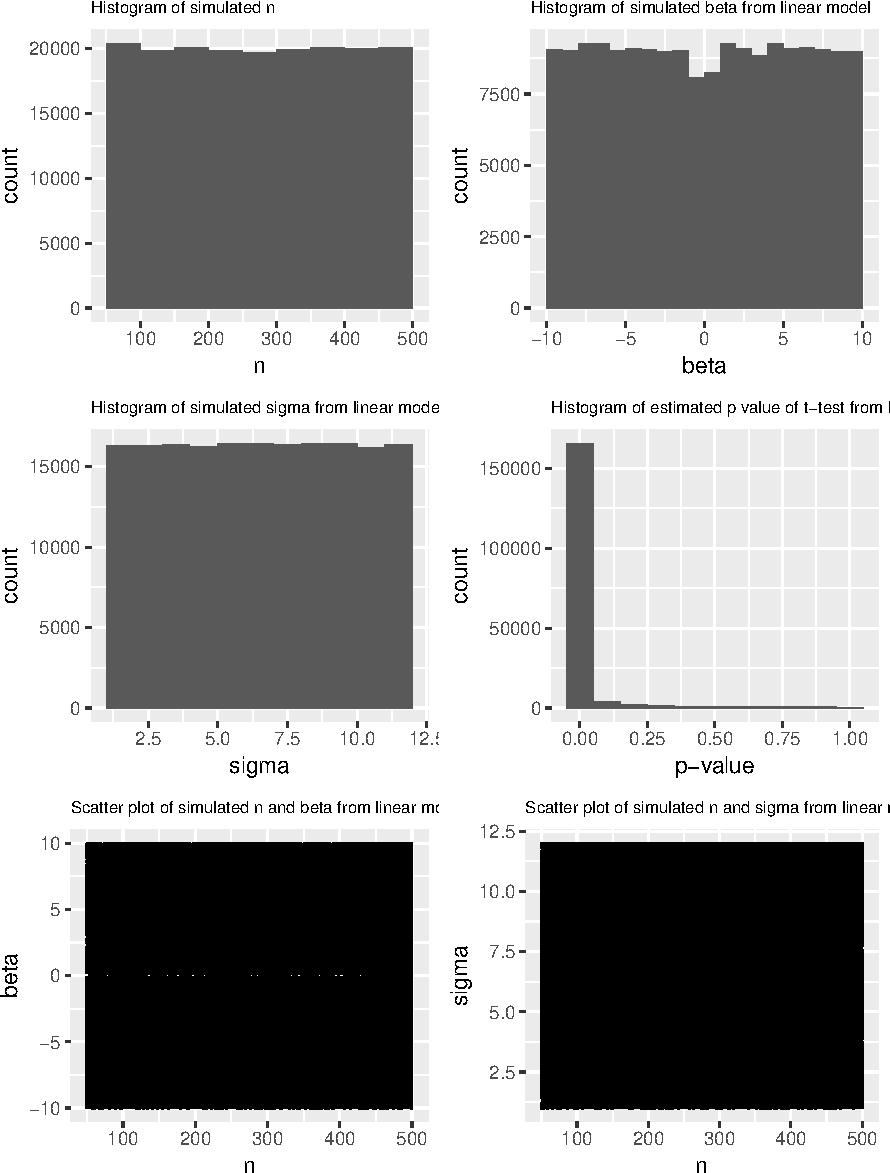
\includegraphics{pc_plots_files/figure-latex/simplot-1.pdf}
\caption{Overview of parameter values used in the linear class
simulation, for computer model training. Good coverage is obtained
across the parameter space.}
\end{figure}

\subsubsection{Null plot simulation}\label{null-plot-simulation}

This is the null scenario in our first experiment, eg. the two variables
under tested are independent of each other. If the data arise from this
situation, then the data plots will not show any systematic patterns
theoretically. It is true that there must be some undesired patterns
formed out of randomness, especially when the sample size is small.
Unlike what Simchoni did in his post, no conventional tests will be used
to sort out the ``significant/insignificant'' samples. Because the
answer to the question that if the deep learning model can distinguish
from patterns formed by chance and by nature is also interesting. The
model is designed the same as the linear model:
\[Y_i = \beta_0 + \beta_1 X_{i}  + \varepsilon_i, ~~i=1, \dots , n\]
with elements of the model generated using the same specification as the
linear model, except\\
- \(\beta_1 = 0\)

e.g.~the coefficient of \(X_i\) is always zero. So \(X\) and \(Y\) are
uncorrelated of each other.

Figure \ref{fig:norela} are four example plots generated using the
specifications above. Same as the linear model simulation, a total
number of 240,000 datasets are simulated under this structure. Figure
\ref{fig:simp} contains a histogram of the simulated n, a histogram of
the simulated \(\sigma\), a histogram of the estimated sample p-value
and a scatter plot of \(\sigma\) against n. These plots show good
coverage over the null parameter space. All simulated data and
associated parameters including estimated sample p-values of t-test are
saved and are used later on for calculating the performance of
conventional t-test.

\begin{figure}
\centering
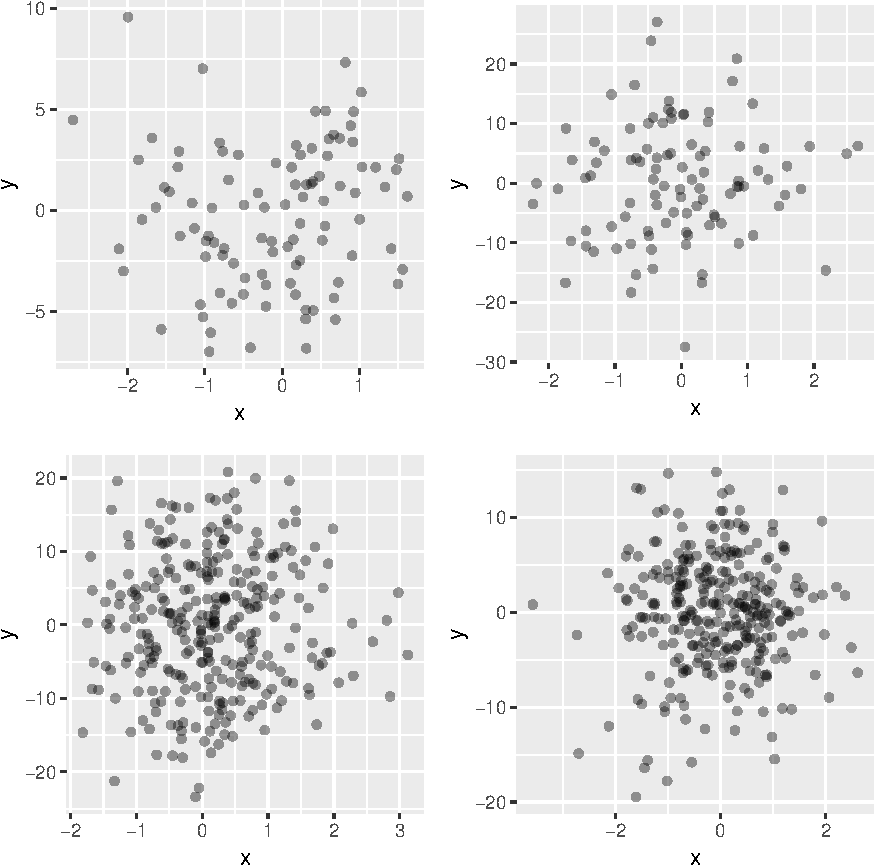
\includegraphics{pc_plots_files/figure-latex/norela-1.pdf}
\caption{Four examples of data plots generated with two independent
variables}
\end{figure}

\begin{figure}
\centering
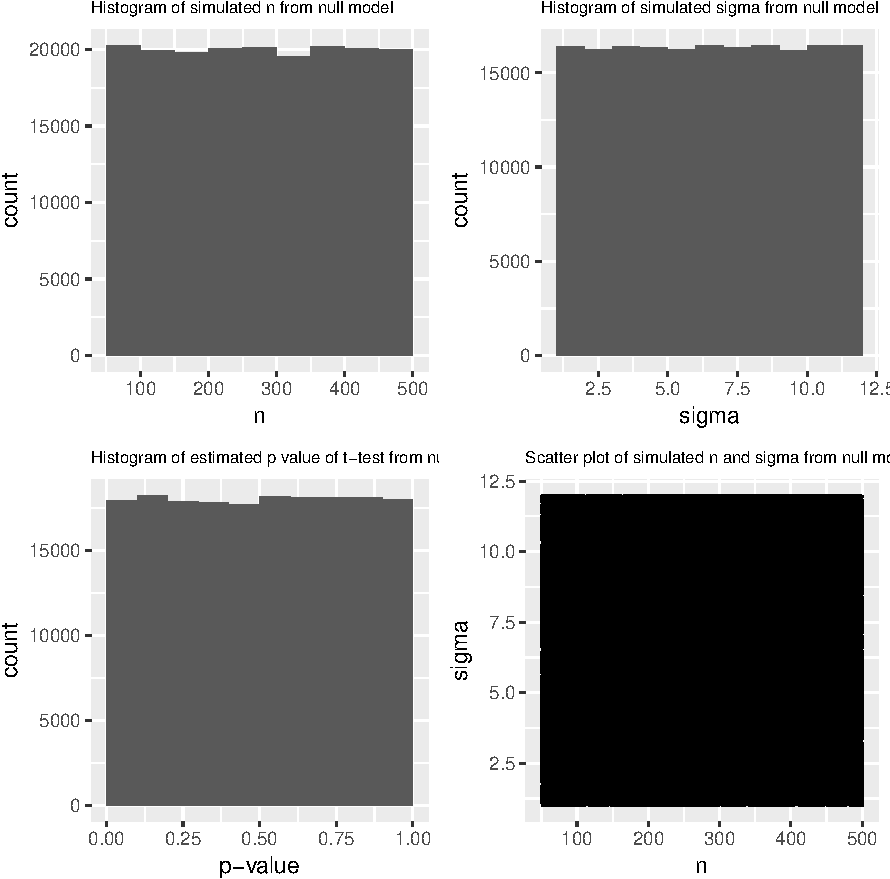
\includegraphics{pc_plots_files/figure-latex/simp-1.pdf}
\caption{Overview of parameter values used in the null class simulation,
for computer model training. Good coverage is obtained across the
parameter space.}
\end{figure}

\subsubsection{Computer model}\label{computer-model}

All convolutional neural network related work is done by the Keras
\citep{keras} package in R \citep{R}, which interfaces to the python
software. The plots used for training and testing in this section is the
scatterplot between the dependent variable Y and the independent
variable X. It can also be considered as the residual plot of such data
fitting to a constant model. The R package ggplot2 \citep{ggplot2} is
used to generate the plots. All plots are resized to \(150\times 150\)
pixel and saved as png. This size is similar to the plot size used in
the lineup for human evaluation. As for the labels given to each image,
we use the true population as the samples' identification directly.

As mentioned above, 240,000 data sets are generated for each of the two
groups in the first experiment. 100,000 of them are set apart for
training. Another 40,000 of the data sets are set apart as the
validation set in order to monitor during training the accuracy of the
model on data it has never seen before. And the leftover (100,000 data
sets) become the unseen test set. We make the test set so large that we
can compare the performance of the convnet with the conventional t-test
properly.

``A convnets takes as input tensors of shape (image height, image width,
image channels).''\citep{DLR18} The channels are normally equal to three
for RGB. In our case, the input tensors are of shape
\(150 \times 150 \times 1\). The channel is equal to one because the
input data is grayscale images. Therefore, the convnet will be
configured to process inputs of size (150, 150, 1). We'll do this by
passing the argument input\_shape = c(150, 150, 1) to the first layer.
The R codes below are used to build the convnets in R. From figure
\ref{modelstruc}, the output shape changes after every layer of ``conv''
and ``pooling'' operations. The original \(150 \times 150 \times 1\)
image is finally sliced into a \(7 \times 7 \times 128\) object (3D
tensor). The figure \ref{diagconv} describes how ``convolution'' and
``max pooling'' operation works. By ``convolution'' the image matrix is
multiplied by a filter, different filter gives different output matrix
which extracting different features from the image. Max pooling select
the max number within a certain area. Then we need to flatten these 3D
tensor into 1D tensor so that they can be processed by the ``sigmoid''
function in the end. The ``sigmoid'' is, in fact, a special case of
logistic function. \(S(\textbf{x})=\frac{1}{1+e^{-\textbf{x}}}\). From
this model structure, we can also see that a total number of 3,452,545
parameters need to be estimated, this is done by gradient descent. 10
epochs (1 epoch = 1 iteration over all samples) are done for training in
our first experiment. The model specifications given by each epoch are
saved, the one gives the overall highest accuracy is chosen to represent
the computer.

\begin{Shaded}
\begin{Highlighting}[]
\KeywordTok{library}\NormalTok{(keras)}
\NormalTok{model <-}\StringTok{ }\KeywordTok{keras_model_sequential}\NormalTok{() }\OperatorTok
\StringTok{  }\KeywordTok{layer_conv_2d}\NormalTok{(}\DataTypeTok{filters =} \DecValTok{32}\NormalTok{, }\DataTypeTok{kernel_size =} \KeywordTok{c}\NormalTok{(}\DecValTok{3}\NormalTok{, }\DecValTok{3}\NormalTok{), }
                \DataTypeTok{activation =} \StringTok{"relu"}\NormalTok{,}
                \DataTypeTok{input_shape =} \KeywordTok{c}\NormalTok{(}\DecValTok{150}\NormalTok{, }\DecValTok{150}\NormalTok{, }\DecValTok{1}\NormalTok{)) }\OperatorTok
\StringTok{  }\KeywordTok{layer_max_pooling_2d}\NormalTok{(}\DataTypeTok{pool_size =} \KeywordTok{c}\NormalTok{(}\DecValTok{2}\NormalTok{, }\DecValTok{2}\NormalTok{)) }\OperatorTok
\StringTok{  }\KeywordTok{layer_conv_2d}\NormalTok{(}\DataTypeTok{filters =} \DecValTok{64}\NormalTok{, }\DataTypeTok{kernel_size =} \KeywordTok{c}\NormalTok{(}\DecValTok{3}\NormalTok{, }\DecValTok{3}\NormalTok{), }
                \DataTypeTok{activation =} \StringTok{"relu"}\NormalTok{) }\OperatorTok
\StringTok{  }\KeywordTok{layer_max_pooling_2d}\NormalTok{(}\DataTypeTok{pool_size =} \KeywordTok{c}\NormalTok{(}\DecValTok{2}\NormalTok{, }\DecValTok{2}\NormalTok{)) }\OperatorTok
\StringTok{  }\KeywordTok{layer_conv_2d}\NormalTok{(}\DataTypeTok{filters =} \DecValTok{128}\NormalTok{, }\DataTypeTok{kernel_size =} \KeywordTok{c}\NormalTok{(}\DecValTok{3}\NormalTok{, }\DecValTok{3}\NormalTok{), }
                \DataTypeTok{activation =} \StringTok{"relu"}\NormalTok{) }\OperatorTok
\StringTok{  }\KeywordTok{layer_max_pooling_2d}\NormalTok{(}\DataTypeTok{pool_size =} \KeywordTok{c}\NormalTok{(}\DecValTok{2}\NormalTok{, }\DecValTok{2}\NormalTok{)) }\OperatorTok
\StringTok{  }\KeywordTok{layer_conv_2d}\NormalTok{(}\DataTypeTok{filters =} \DecValTok{128}\NormalTok{, }\DataTypeTok{kernel_size =} \KeywordTok{c}\NormalTok{(}\DecValTok{3}\NormalTok{, }\DecValTok{3}\NormalTok{), }
                \DataTypeTok{activation =} \StringTok{"relu"}\NormalTok{) }\OperatorTok
\StringTok{  }\KeywordTok{layer_max_pooling_2d}\NormalTok{(}\DataTypeTok{pool_size =} \KeywordTok{c}\NormalTok{(}\DecValTok{2}\NormalTok{, }\DecValTok{2}\NormalTok{)) }\OperatorTok
\StringTok{  }\KeywordTok{layer_flatten}\NormalTok{() }\OperatorTok
\StringTok{  }\KeywordTok{layer_dense}\NormalTok{(}\DataTypeTok{units =} \DecValTok{512}\NormalTok{, }\DataTypeTok{activation =} \StringTok{"relu"}\NormalTok{) }\OperatorTok
\StringTok{  }\KeywordTok{layer_dense}\NormalTok{(}\DataTypeTok{units =} \DecValTok{1}\NormalTok{, }\DataTypeTok{activation =} \StringTok{"sigmoid"}\NormalTok{)}
\end{Highlighting}
\end{Shaded}

\begin{figure*}[h]
\centerline{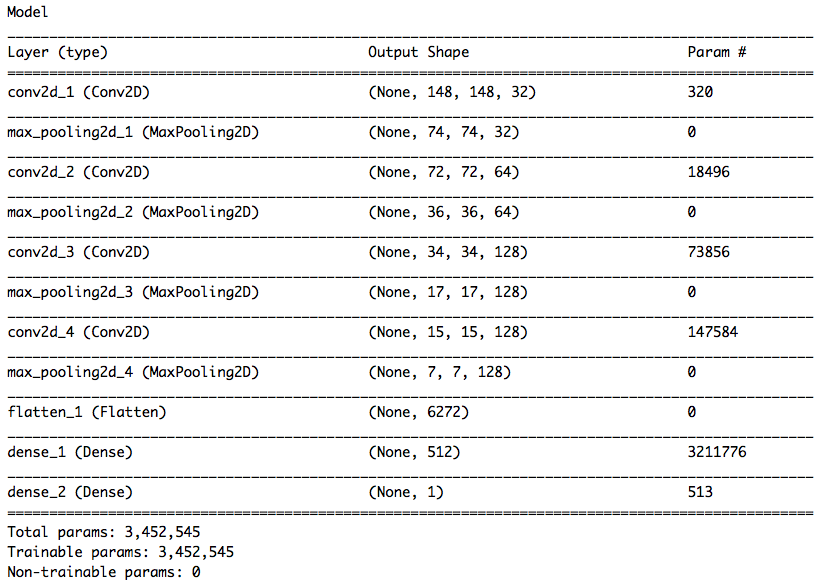
\includegraphics[width=15cm]{figures/modelstruc.png}}
\caption{The deep learning model structure used for both of the experiments.}
\label{modelstruc}
\end{figure*}

\begin{figure*}[h]
\centerline{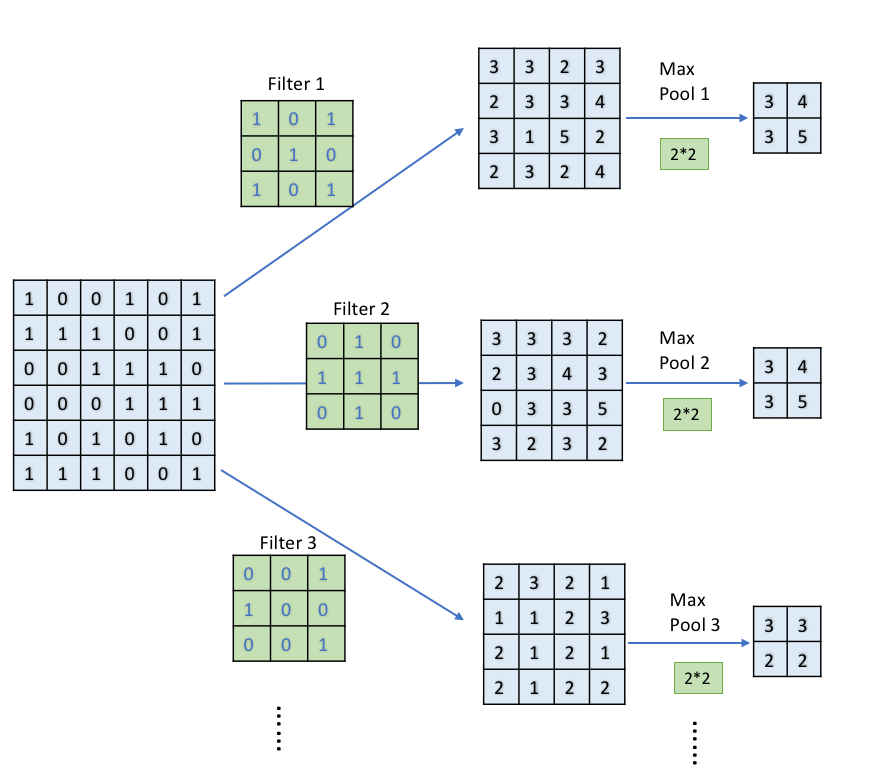
\includegraphics[width=15cm]{figures/diagconv.png}}
\caption{Illustration of convolution and pooling steps on an image. The convolution step applies a fixed number of filters to sliding windows of $3\times 3$ cells. Pooling applies a statistic to distinct $2\times 2$ tiling of the image. In our model, the statistic used is the maximum of the four values. These transformations are the pre-processing steps done on every image in the training sample, to fit the model, and also to the validation and test images prior to prediction. }
\label{diagconv}
\end{figure*}

The plot of the training history (figure \ref{histlinear}) shows high
accuracy achieved in both train and validation set (93\%-94\%); slight
overfitting starts from the fourth epoch; the variation of the values of
accuracy and loss in validation set are very small after the fourth
epoch. Hence, both our convnets and dataset are large enough and the
training of our first experiment can be concluded. Then we select the
fourth, sixth, eighth and the tenth model to have them tested on the
unseen test set. And the results are shown in the table
\ref{checkpoints}. In this table, the ``\(1-\alpha\)'' means the
accuracy of each computer model tested on the ``null data'' in the test
set only. \(\alpha\) here is an analogy to the Type I error in the
conventional hypothesis test. Similarly, the ``power'' is the accuracy
of each computer model tested on the ``linear data'' in the test set
only. The t-test performance in this table is calculated at 5\%
significance level.

The 8th model is chosen according to the overall accuracy on the test
set. We should note that since the majority of the data plots in Turk's
experiment have been generated from linear relationships (when the
alternative hypothesis is true), it is a disadvantage for the computer
comparing in terms of being tested on the Turk's data. Because of the
difference in \(\alpha\) (\(\alpha \approx 0.02\) for the 8th computer
model) the 5\% significant t-test and 5\% human evaluations may have
higher power than the computer model.

\begin{table}[ht]
\begin{center}
\begin{tabular}{|l|rrr|}\hline
Tests & Linear & Null & Overall \\\hline
4 epoch & 0.892 & 0.984 &  0.938 \\   
6 epoch & 0.889 & 0.986 & 0.937 \\
8 epoch & 0.896 & 0.981 & 0.939 \\
10 epoch & 0.904 & 0.971 & 0.938 \\
5\% $t$-test & 0.921 & 0.949 & 0.935\\\hline
\end{tabular}
\end{center}
\caption{Performance of four checkpoints from the {\em convnets} model, and the 5\% significant $t$-test, computed on the test set. Accuracy is reported for each class, and overall. There is a slight improvement as the number of epochs increases, with 10 epochs being reasonably close to the ideal $t$-test accuracy.}
\label{checkpoints}
\end{table}

\section{Results}
\label{sec:results}

The performance of the computer model for the Turk study data is tested
in three steps:

\begin{itemize}
\item
  Re-generate the 70 ``real plots'' using the same data in Turk study
  (without null plots);
\item
  Create a separate test directory for the 70 ``real plots''
  exclusively;
\item
  The computer model's predicted accuracy over the 70 ``real plots'' is
  recorded as the model's performance.
\end{itemize}

The conclusion of human evaluation is obtained differently from the
computers. Because human evaluated ``lineup'', not only the ``real
plots''. The performance is tested in five steps:

\begin{itemize}
\item
  Count the total number of evaluations made by human for one lineup (N)
  and the number of correct answers for that lineup (k);
\item
  Obtain N and k for all 70 lineups;
\item
  Calculate p-value associated with each real plot using the formula
  introduced in section 2 of \citet{MM13};
\item
  Draw the conclusion: reject the null when the calculated p-value is
  smaller than \(\alpha\).
\item
  The accuracy of the conclusions the 70 real plots is presenting for
  the human performance.
\end{itemize}

For a fair competition, the Type I error (\(\alpha\)) should be held the
same for all test methods. However, we do not have direct control over
the \(\alpha\) of the computer model. Because the \(\alpha\) estimated
from the computer model is close to 2\%. Therefore, 2\% significant
t-test and 2\% significant human conclusion are also included to give a
complete picture of the comparison. The comparing result (table 2.3) is
interesting. Human achieves the highest accuracy, and the conclusion
from the human evaluation is robust to smaller p-values; 5\% significant
t-test is the second best, 2\% significant t-test and the computer model
give the same results.

\begin{longtable}[]{@{}cccc@{}}
\caption{Accuracy of testing the 70 data plots evaluated by human
computer and the conventional t-test.}\tabularnewline
\toprule
\begin{minipage}[b]{0.09\columnwidth}\centering\strut
Rank\strut
\end{minipage} & \begin{minipage}[b]{0.17\columnwidth}\centering\strut
Tests\strut
\end{minipage} & \begin{minipage}[b]{0.21\columnwidth}\centering\strut
No. of correct\strut
\end{minipage} & \begin{minipage}[b]{0.12\columnwidth}\centering\strut
Accuracy\strut
\end{minipage}\tabularnewline
\midrule
\endfirsthead
\toprule
\begin{minipage}[b]{0.09\columnwidth}\centering\strut
Rank\strut
\end{minipage} & \begin{minipage}[b]{0.17\columnwidth}\centering\strut
Tests\strut
\end{minipage} & \begin{minipage}[b]{0.21\columnwidth}\centering\strut
No. of correct\strut
\end{minipage} & \begin{minipage}[b]{0.12\columnwidth}\centering\strut
Accuracy\strut
\end{minipage}\tabularnewline
\midrule
\endhead
\begin{minipage}[t]{0.09\columnwidth}\centering\strut
1\strut
\end{minipage} & \begin{minipage}[t]{0.17\columnwidth}\centering\strut
Human 5\%\strut
\end{minipage} & \begin{minipage}[t]{0.21\columnwidth}\centering\strut
47\strut
\end{minipage} & \begin{minipage}[t]{0.12\columnwidth}\centering\strut
0.6714\strut
\end{minipage}\tabularnewline
\begin{minipage}[t]{0.09\columnwidth}\centering\strut
1\strut
\end{minipage} & \begin{minipage}[t]{0.17\columnwidth}\centering\strut
Human 2\%\strut
\end{minipage} & \begin{minipage}[t]{0.21\columnwidth}\centering\strut
47\strut
\end{minipage} & \begin{minipage}[t]{0.12\columnwidth}\centering\strut
0.6714\strut
\end{minipage}\tabularnewline
\begin{minipage}[t]{0.09\columnwidth}\centering\strut
2\strut
\end{minipage} & \begin{minipage}[t]{0.17\columnwidth}\centering\strut
T-test 5\%\strut
\end{minipage} & \begin{minipage}[t]{0.21\columnwidth}\centering\strut
43\strut
\end{minipage} & \begin{minipage}[t]{0.12\columnwidth}\centering\strut
0.6143\strut
\end{minipage}\tabularnewline
\begin{minipage}[t]{0.09\columnwidth}\centering\strut
3\strut
\end{minipage} & \begin{minipage}[t]{0.17\columnwidth}\centering\strut
Computer 2\%\strut
\end{minipage} & \begin{minipage}[t]{0.21\columnwidth}\centering\strut
39\strut
\end{minipage} & \begin{minipage}[t]{0.12\columnwidth}\centering\strut
0.5571\strut
\end{minipage}\tabularnewline
\begin{minipage}[t]{0.09\columnwidth}\centering\strut
4\strut
\end{minipage} & \begin{minipage}[t]{0.17\columnwidth}\centering\strut
T-test 2\%\strut
\end{minipage} & \begin{minipage}[t]{0.21\columnwidth}\centering\strut
39\strut
\end{minipage} & \begin{minipage}[t]{0.12\columnwidth}\centering\strut
0.5571\strut
\end{minipage}\tabularnewline
\bottomrule
\end{longtable}

\subsection{Aside discussion}\label{aside-discussion}

Under the condition specified in this chapter, the conventional t-test
is supposed to be the uniformly most powerful (UMP) test in terms of
detecting the linear relationship according to the Neyman--Pearson
lemma. \citep{Neyman289} Although human achieved the best performance in
the Turk experiment dataset, it does not mean computer does badly since
the Turk experiment dataset only contains 70 plots. As we can see from
table \ref{checkpoints}, t-test and convnets behave quite similarly on
both the test data and Turk's experiment data. Given our test set is
large enough (200,000 images totally), it is reasonable to assume that
the convnets is, in fact, implementing the t-test or trying to approach
the t-test. In other words, the best strategy the convnets learned, in
this case, may turn out to be t-test.

To check this idea, we calculated the accuracy of t-test again, with
different \(\alpha\) (from 0.005 to 0.1 with 0.005 increments) on all
200,000 test sets. The estimated power and overall accuracy were
recorded. When \(\alpha=0.015\), the overall accuracy reaches its
maximum. This value approximately coincides with the \(\alpha\) chosen
by the convnets. And since the \(\alpha\) of convnets is from 0.0142 to
0.0347 on the test set, we truncated the t-test data to create figure
\ref{fig:ttdl}. The upper dots represent overall accuracy achieved by
convnets (red) and t-test (green), while the lower dots stand for the
estimated power in the test set. The smooth line overlaid aids the eye
in seeing patterns. From this graph, we can see the convnets and t-test
perform very similarly, while t-test has overall better performance.

\begin{figure*}[h]
\centerline{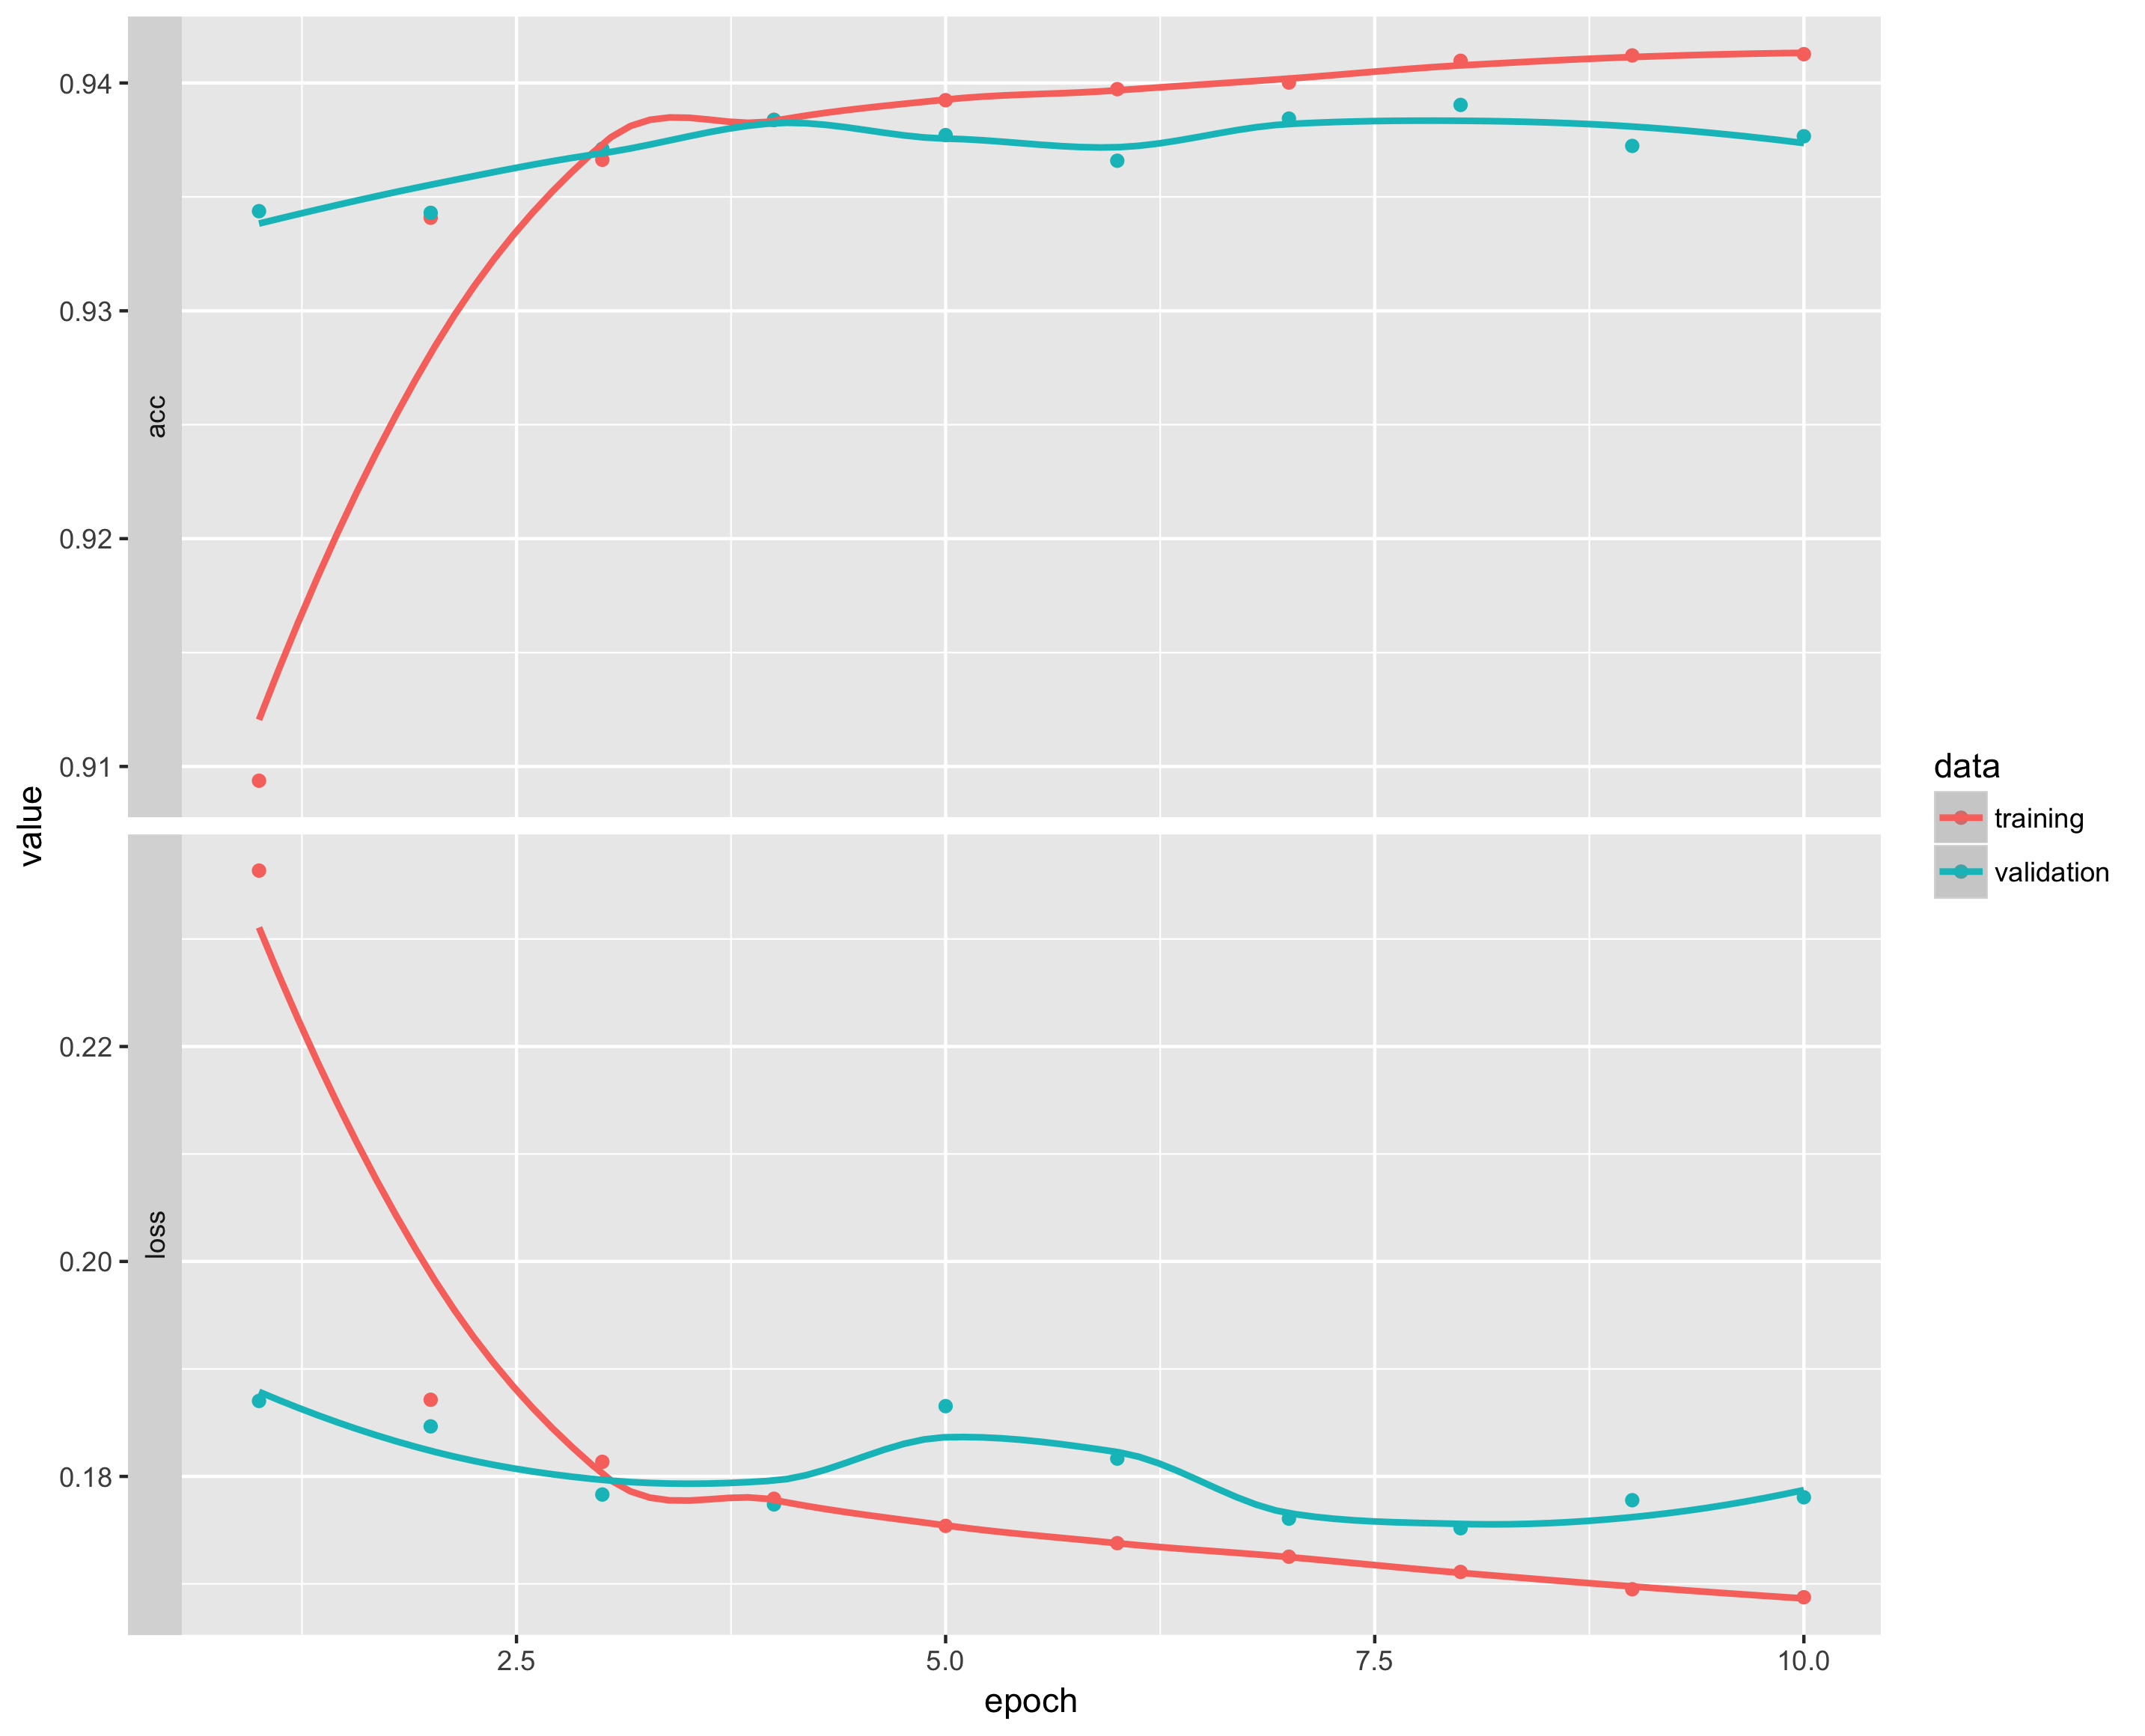
\includegraphics[width=15cm]{figures/linear_history_plot.png}}
\caption{Training and validation metrics of linear vs. null model in our first experiment. The top plot is the accuracy achieved in train and validaton sets, while the bottom plot is the loss. Red presents model performance in train set while green presents validation.}
\label{histlinear}
\end{figure*}

\begin{figure}

{\centering 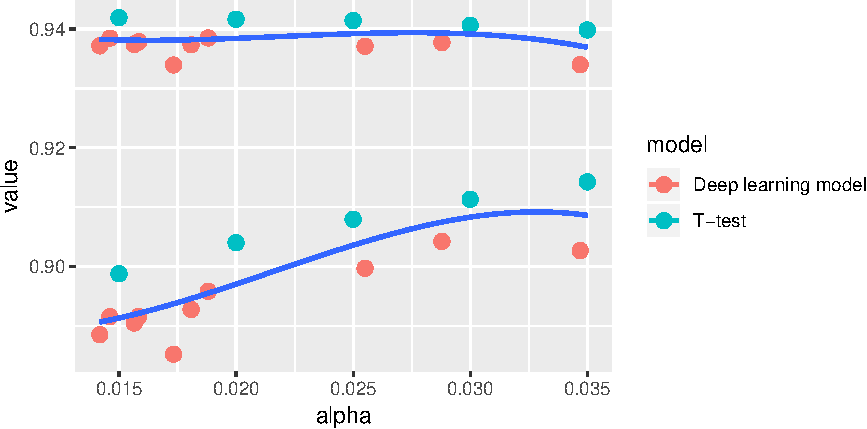
\includegraphics{pc_plots_files/figure-latex/ttdl-1} 

}

\caption{Comparison between computer model and t-test for alpha in (0.01, 0.04), they perform very similarly, but t-test has overall better performance.}\label{fig:ttdl}
\end{figure}

\bibliographystyle{agsm}
\bibliography{bibliography.bib}

\end{document}
